\documentclass[10pt,letterpaper]{article}
\usepackage[margin=0.72in]{geometry}
\usepackage[T1]{fontenc}
\usepackage{mathptmx}
\usepackage{microtype}
\usepackage{amsmath,amssymb}
\usepackage{xcolor}
\usepackage{titlesec}
\usepackage{graphicx}
\usepackage{booktabs}
\usepackage{tabularx}
\usepackage{enumitem}
\usepackage{tikz}
\usetikzlibrary{positioning,arrows.meta}
\usepackage[font=small,labelfont=bf,skip=3pt]{caption}
\usepackage[hidelinks]{hyperref}
\usepackage{xurl}
\definecolor{ink}{HTML}{20364A}
\titleformat{\section}{\normalsize\bfseries\color{ink}}{\arabic{section}.}{0.5em}{}
\titleformat{\subsection}{\small\bfseries\color{ink}}{}{0em}{}
\titlespacing*{\section}{0pt}{7pt}{2pt}
\titlespacing*{\subsection}{0pt}{5pt}{1pt}
\setlength{\parindent}{0pt}
\setlength{\parskip}{4pt}
\setlength{\emergencystretch}{2em}
\setlength{\abovedisplayskip}{3pt}
\setlength{\belowdisplayskip}{3pt}
\setlength{\textfloatsep}{8pt}
\setlength{\floatsep}{6pt}
\setlist{nosep, leftmargin=1.2em}
\newcommand{\answer}[1]{\textbf{\color{ink}Answer: #1}}
\urlstyle{same}
\pagestyle{plain}

\begin{document}
\begin{center}
{\Large\bfseries Can We Forecast Price Impact? Kyle's $\lambda$ Minute by Minute}\\[3pt]
{\small MSCF 46982 Market Microstructure and Algorithmic Trading, Final Paper \quad$\cdot$\quad Andrew IDs: samayp, [teammates]}
\end{center}
\vspace{-4pt}

\begin{abstract}
\noindent\small
When a trader buys, the price moves against them; Kyle's $\lambda$ measures by how much. We ask whether $\lambda$ can be forecast from market conditions one minute earlier, and whether that forecast helps someone executing a large order. Using one-minute NYSE TAQ data for the 30 Dow stocks in February 2020, processed in kdb+, we find that only the unexpected part of order flow moves prices; that impact in the first half hour is nearly twice its midday level; and that wide spreads raise impact while deep order books lower it. Forecasting impact this way improves out-of-sample fit, and most of a machine-learning model's extra accuracy comes from one simple fact: impact grows more slowly than order size. The forecast does not help a trader decide \emph{when} to trade within an hour, but it does help them estimate \emph{how much} an order will cost, cutting the error of that estimate by 10\%.
\end{abstract}

\section{Introduction}
A fund that needs to buy \$50 million of a stock cannot do it in one trade; it splits the order and buys over an hour or a day. Every purchase pushes the price up, so the cost of the order depends on how sensitive the price is to buying pressure at the moment of each trade. Kyle (1985) calls this sensitivity $\lambda$. Most practitioners treat $\lambda$ as a constant for each stock, but its drivers (how much private information is around, how much ordinary trading there is to hide in) clearly change during the day. If $\lambda$ moves with conditions we can observe, it should be forecastable, and a forecast should be worth something to a trader. Hasbrouck and Seppi (2001) and Kwan, Philip and Shkilko (2021) document time variation in liquidity and price discovery; we go a step further and ask whether that variation can be forecast and used.

We organise the paper around five questions, listed in Table~\ref{tab:questions}. The first three test what theory says should move $\lambda$; the last two ask whether a forecast of $\lambda$ is accurate, and whether it is useful.

\begin{table}[h]
\centering\small
\caption{The five questions of this paper. Answers are in Section~\ref{sec:results}.}\label{tab:questions}
\begin{tabularx}{\textwidth}{@{}p{4.4cm}XX@{}}
\toprule
Question & What theory predicts & How we test it \\
\midrule
\textbf{1. Surprise flow.} Does order flow that could have been predicted still move prices? & No: a market maker who expects the flow has already priced it in (Hasbrouck, 1991). & Split each minute's flow into a forecast and a surprise; regress the price change on both. \\
\textbf{2. Time of day.} Is impact highest at the open? & Yes: overnight news is absorbed early in the day (Admati and Pfleiderer, 1988). & Estimate $\lambda$ separately for each half hour; test whether they are equal. \\
\textbf{3. Market conditions.} Do wide spreads and thin order books raise impact? & Yes: both signal more informed trading or less liquidity (Kyle, 1985; Glosten and Milgrom, 1985). & Let $\lambda$ depend on the previous minute's spread, depth, volatility and activity. \\
\textbf{4. Forecasting.} Can impact be forecast out of sample, and is machine learning worth it? & A condition-dependent $\lambda$ should beat a constant one. & Train on Feb 3--14, test on Feb 18--28; compare a regression with gradient boosting. \\
\textbf{5. Value to a trader.} Does the forecast help execute a large order? & It should help both to time trades and to estimate their cost (Almgren and Chriss, 2000). & Simulate 1,620 one-hour orders; compare schedules and cost estimates with simple benchmarks. \\
\bottomrule
\end{tabularx}
\end{table}

\section{Why impact should vary}
In Kyle's model an informed trader knows the asset's value $v \sim N(p_0, \sigma_v^2)$ and submits an order $x = \beta(v - p_0)$; noise traders add $u \sim N(0, \sigma_u^2)$. The market maker sees only the total $y = x + u$ and sets $p = p_0 + \lambda y$. The informed trader's best response is $\beta = 1/2\lambda$, and a competitive market maker sets $\lambda = \operatorname{Cov}(v, y)/\operatorname{Var}(y)$. Solving the two together gives
\begin{equation}
\Delta p = \lambda \, y, \qquad \lambda = \frac{\sigma_v}{2\,\sigma_u}.
\end{equation}
Impact is high when there is a lot of private information ($\sigma_v$ large) and low when there is plenty of noise trading to hide in ($\sigma_u$ large). Two refinements complete the picture. Glosten and Milgrom (1985) show that the bid--ask spread is the market maker's protection against informed traders, so a wide spread signals a high $\lambda$. Hasbrouck (1991) argues that only the \emph{unexpected} part of order flow carries news. These three ideas give the predictions in Table~\ref{tab:questions}.

\section{Data}
We use NYSE TAQ trades and best quotes (NBBO) for the 30 Dow stocks over all 19 trading days on the course kdb+ server, February 3--28, 2020. Figure~\ref{fig:pipeline} shows the pipeline. All heavy work runs on the server in q: each trade is matched to the quote in force at that moment with an as-of join, and signed as a buy or a sell with the Lee and Ready (1991) rule. Every column of the q output is checked against an independent pandas implementation.

\begin{figure}[h]
\centering
% Data pipeline diagram, included by report.tex.
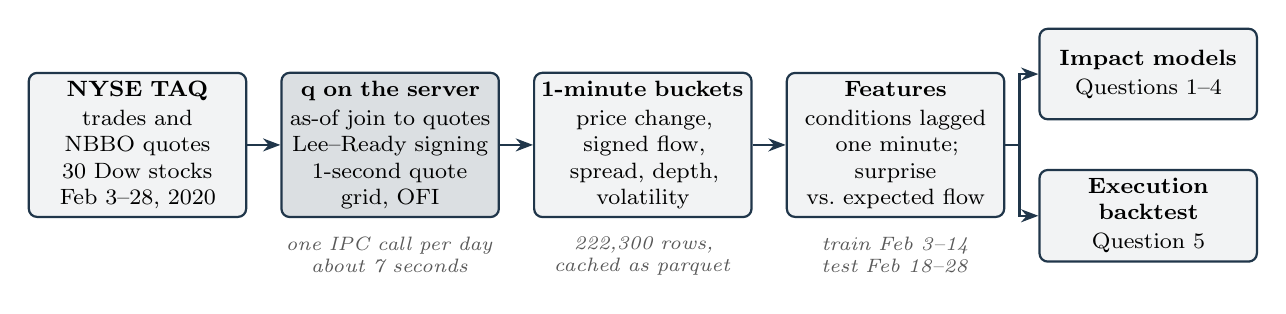
\begin{tikzpicture}[
  node distance=0.42cm,
  box/.style={draw=ink, rounded corners=3pt, thick, fill=ink!6, align=center,
              text width=2.55cm, minimum height=1.75cm, font=\footnotesize, inner sep=3pt},
  hot/.style={box, fill=ink!16},
  note/.style={font=\scriptsize\itshape, text=black!65, align=center, text width=2.6cm},
  arrow/.style={-{Stealth[length=2.2mm]}, thick, draw=ink}
]
\node[box] (taq) {\textbf{NYSE TAQ}\\[1pt] trades and NBBO quotes\\ 30 Dow stocks\\ Feb 3--28, 2020};
\node[hot, right=of taq] (q) {\textbf{q on the server}\\[1pt] as-of join to quotes\\ Lee--Ready signing\\ 1-second quote grid, OFI};
\node[box, right=of q] (buckets) {\textbf{1-minute buckets}\\[1pt] price change, signed flow,\\ spread, depth, volatility};
\node[box, right=of buckets] (features) {\textbf{Features}\\[1pt] conditions lagged\\ one minute; surprise\\ vs.\ expected flow};
\node[box, right=of features, yshift=0.9cm, minimum height=1.15cm] (models) {\textbf{Impact models}\\[1pt] Questions 1--4};
\node[box, right=of features, yshift=-0.9cm, minimum height=1.15cm] (exec) {\textbf{Execution backtest}\\[1pt] Question 5};
\draw[arrow] (taq) -- (q);
\draw[arrow] (q) -- (buckets);
\draw[arrow] (buckets) -- (features);
\draw[arrow] (features.east) -- ++(0.18,0) |- (models.west);
\draw[arrow] (features.east) -- ++(0.18,0) |- (exec.west);
\node[note, below=0.12cm of q] {one IPC call per day\\ about 7 seconds};
\node[note, below=0.12cm of buckets] {222,300 rows,\\ cached as parquet};
\node[note, below=0.12cm of features] {train Feb 3--14\\ test Feb 18--28};
\end{tikzpicture}

\caption{Data pipeline. Millions of quote updates per day are reduced to one row per stock per minute on the server.}\label{fig:pipeline}
\end{figure}

We train on February 3--14 and test on February 18--28. The test period contains a calm week and the first week of the COVID-19 sell-off, which Table~\ref{tab:summary} shows was a very different market: volume and quote traffic more than doubled, spreads widened by 65\% and volatility rose 2.4 times. We report results for both weeks.

\begin{table}[h]
\centering\small
\caption{Summary statistics, averages per stock and day.}\label{tab:summary}
\setlength{\tabcolsep}{5pt}
\begin{tabular}{lrrrrrr}
\toprule
 & Days & Volume (M shares) & Trades (k) & Spread (bps) & Depth (lots) & 1-min volatility (bps) \\
\midrule
Training, Feb 3--14 & 10 & 7.66 & 71.1 & 2.19 & 35.1 & 5.14 \\
Test, calm week, Feb 18--21 & 4 & 7.20 & 67.5 & 2.31 & 35.3 & 5.13 \\
Test, sell-off week, Feb 24--28 & 5 & 16.80 & 164.0 & 3.81 & 22.2 & 12.48 \\
\bottomrule
\end{tabular}
\end{table}

\section{Method}
For each stock and minute $t$ we measure the change in the mid-quote, $\Delta m_t$ (in basis points), and the signed order flow $x_t$ (buy volume minus sell volume, divided by the stock's average one-minute volume so that stocks are comparable). Market conditions $z_{t-1}$ are measured in the \emph{previous} minute, so nothing in a forecast uses information from the minute being forecast. Our main model lets $\lambda$ depend on those conditions:
\begin{equation}
\Delta m_t = \mu + \gamma' z_{t-1} + \underbrace{\Big(\lambda_0 + \textstyle\sum_k \lambda_k z_{k,t-1}\Big)}_{\lambda_t}\, x_t + \varepsilon_t .
\end{equation}
Each $\lambda_k$ answers a plain question: how much more does a unit of flow move the price when condition $k$ is one standard deviation higher? Table~\ref{tab:method} summarises the remaining choices.

\begin{table}[h]
\centering\small
\caption{Method at a glance.}\label{tab:method}
\begin{tabularx}{\textwidth}{@{}p{3.3cm}X@{}}
\toprule
Market conditions $z_{t-1}$ & Spread, quoted depth, volatility over the last 5 minutes, number of trades, number of quote updates, order-flow imbalance at the best quotes (Cont, Kukanov and Stoikov, 2014); all lagged one minute \\
Expected vs.\ surprise flow & Forecast flow from its last 5 minutes (an AR(5) model); the surprise is actual minus forecast \\
Four impact models & \emph{Constant impact} (Kyle); \emph{condition-dependent impact} (equation 2, plus a time-of-day term); \emph{+ square-root term}, adding $\operatorname{sign}(x)\sqrt{|x|}$ (T\'oth et al., 2011); \emph{gradient boosting} (LightGBM; Ke et al., 2017), forced to be increasing in flow \\
No look-ahead & All scaling, the AR(5) model and every model parameter use training days only; gradient-boosting settings are chosen by time-series cross-validation over training days \\
Inference & Standard errors clustered by stock and by date; forecasts compared with the Diebold and Mariano (1995) test \\
\bottomrule
\end{tabularx}
\end{table}

\section{Results}\label{sec:results}

\subsection{Question 1: Does predictable order flow move prices?}
\answer{No. Only the surprise moves prices.} The forecast explains just 1.1\% of the variation in flow, but the split is sharp (Table~\ref{tab:reg}): a unit of surprise flow moves the price by 3.86 bps ($t = 13.1$), while a unit of predictable flow moves it by $-0.41$ bps, which is indistinguishable from zero. The market appears to see through flow it could have anticipated, just as Hasbrouck (1991) predicts.

\begin{table}[h]
\centering\small
\caption{What moves impact (training days). Coefficients in bps per unit of flow, $t$-statistics in parentheses. Conditions are in standard deviations; the third model also includes them on their own.}\label{tab:reg}
\begin{tabular}{lccc}
\toprule
 & Constant impact & Question 1: surprise split & Question 3: market conditions \\
\midrule
Order flow $x_t$ & 3.81 (13.2) & & 3.38 (14.7) \\
\quad expected part $\hat x_t$ & & $-0.41$ ($-0.5$) & \\
\quad surprise part $u_t$ & & 3.86 (13.1) & \\
Flow $\times$ previous spread & & & 0.87 (5.2) \\
Flow $\times$ previous depth & & & $-0.62$ ($-2.0$) \\
Flow $\times$ previous volatility & & & 0.14 (1.0) \\
Flow $\times$ previous activity (trades / quote updates) & & & 0.41 (1.5) / 0.62 (1.3) \\
Flow $\times$ previous order-flow imbalance & & & $-0.09$ ($-1.4$) \\
$R^2$ & 0.106 & 0.107 & 0.119 \\
\bottomrule
\end{tabular}
\end{table}

\subsection{Question 2: Is impact highest at the open?}
\answer{Yes, by a wide margin.} Impact in the first half hour is 6.07 bps per unit of flow, against an average of 3.29 between 12:00 and 14:00 (Figure~\ref{fig:lambda}a). Equal impact across the day is firmly rejected ($p = 0.001$).

\begin{figure}[h]
\centering
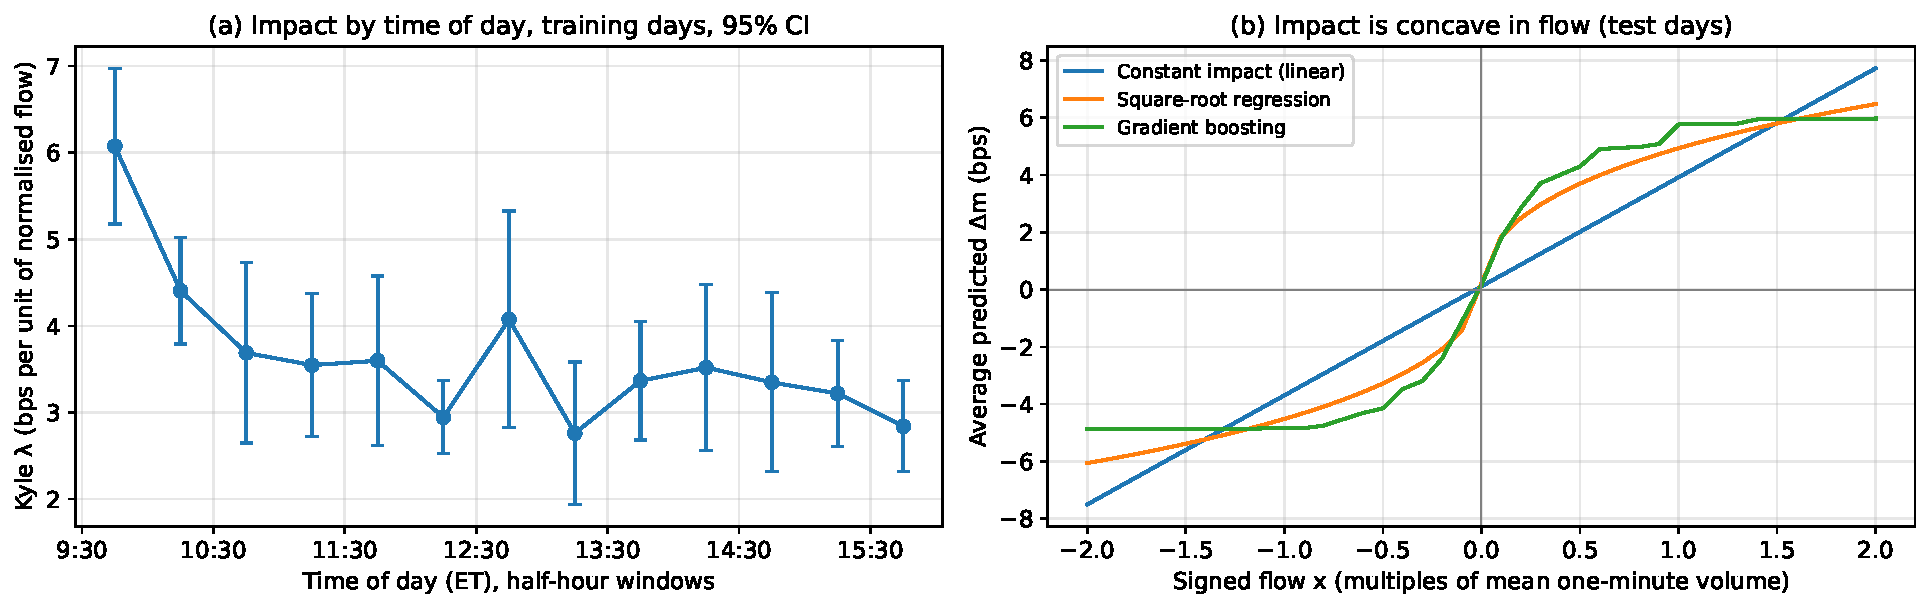
\includegraphics[width=\textwidth]{../figures/fig2_lambda_shape.pdf}
\caption{(a) Kyle's $\lambda$ by half hour, training days, with 95\% confidence intervals. (b) Predicted price change as order flow grows, test days: impact rises steeply for small flows and flattens for large ones, which a straight line (Kyle's model) misses.}\label{fig:lambda}
\end{figure}

\subsection{Question 3: Do wide spreads and thin order books raise impact?}
\answer{Yes for spreads and depth; the other conditions add little.} A one-standard-deviation wider spread in the previous minute raises $\lambda$ by 0.87 ($t = 5.2$), about a quarter of its average; deeper quotes lower it by 0.62 ($t = -2.0$). Both signs match Kyle and Glosten--Milgrom. Volatility, trading activity and order-flow imbalance are not significant once spread and depth are included.

\subsection{Question 4: Can impact be forecast, and is machine learning worth it?}
\answer{Yes, and most of the machine-learning gain comes from one simple feature.} On the nine test days, letting $\lambda$ depend on conditions raises out-of-sample $R^2$ from 7.9\% to 8.9\% (Table~\ref{tab:oos}). The larger step comes from the \emph{shape} of impact: adding a single square-root term lifts $R^2$ to 12.7\%, and gradient boosting adds only one more point, to 13.7\%. Figure~\ref{fig:lambda}b shows why. Impact grows more slowly than order size, and both flexible models learn this; beyond about one minute's typical volume the boosted model flattens because it has seen few such trades. SHAP values (Lundberg and Lee, 2017) in Figure~\ref{fig:shap} confirm that the boosted model relies on the same ingredients as the regression: flow first, then volatility and spread, with flow mattering more when the spread is wide. One extra term in a regression thus recovers about 80\% of the black box's gain while keeping every coefficient interpretable.

\begin{table}[h]
\centering\small
\caption{Out-of-sample fit, test days (Feb 18--28). DM is the Diebold--Mariano statistic against constant impact; negative values favour the model.}\label{tab:oos}
\begin{tabular}{lcccc}
\toprule
Model & $R^2$, all test days & $R^2$, calm week & $R^2$, sell-off week & DM vs.\ constant \\
\midrule
Constant impact (Kyle) & 7.9\% & 9.5\% & 7.7\% & -- \\
Condition-dependent impact & 8.9\% & 10.8\% & 8.6\% & $-4.4$ \\
\quad + square-root term & 12.7\% & 17.2\% & 12.0\% & $-15.5$ \\
Gradient boosting & 13.7\% & 18.8\% & 12.9\% & $-13.8$ \\
\bottomrule
\end{tabular}
\end{table}

\begin{figure}[h]
\centering
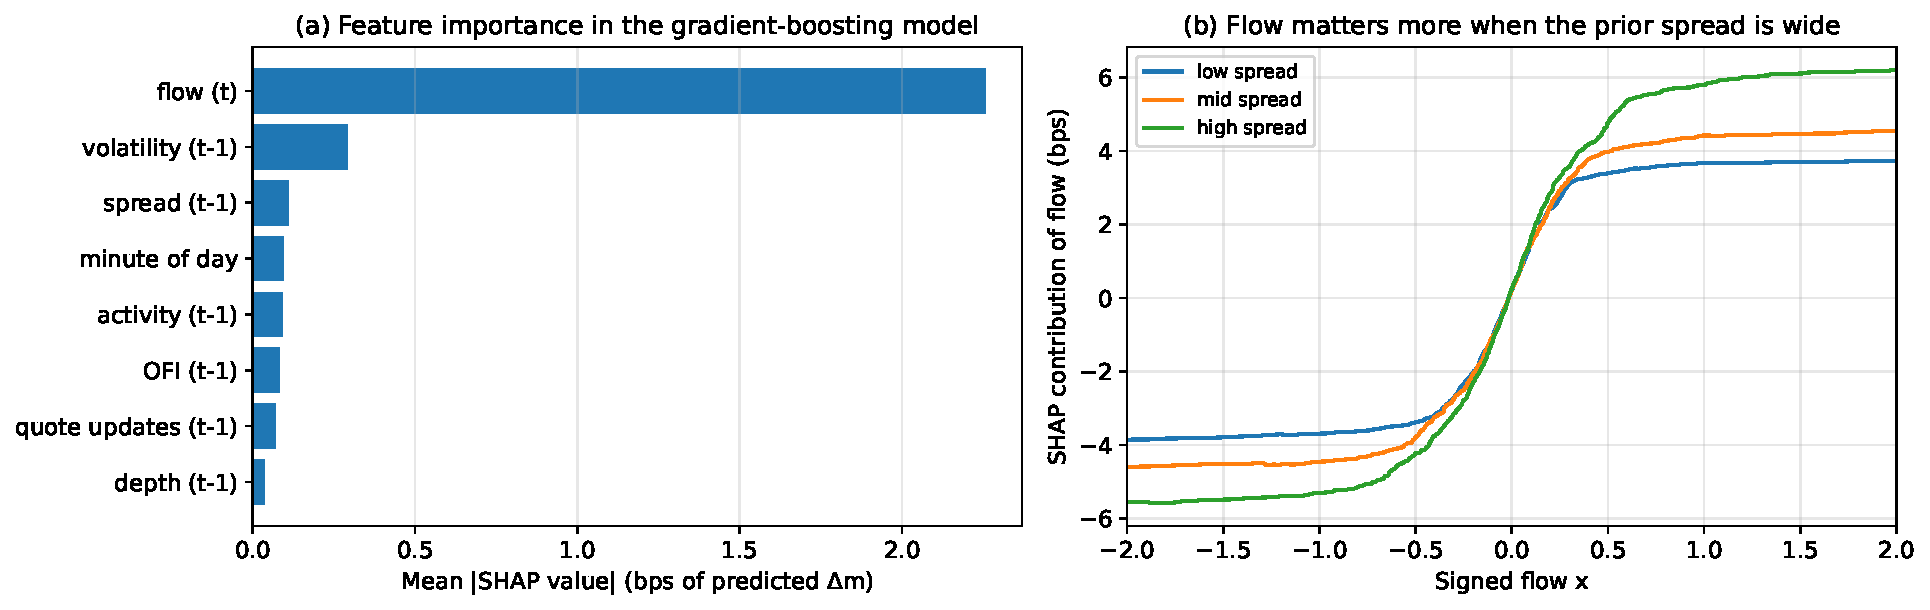
\includegraphics[width=\textwidth]{../figures/fig3_shap.pdf}
\caption{Inside the gradient-boosting model, test days. (a) Average contribution of each input to the predicted price change. (b) Contribution of order flow, by how wide the spread was in the previous minute.}\label{fig:shap}
\end{figure}

\subsection{Question 5: Does the forecast help a trader execute a large order?}
\answer{Not for timing trades within the hour; yes for estimating what the order will cost.}

\textit{Setup.} We simulate buying 5\% of a stock's daily volume over one hour (about \$52.6 million for the average stock), starting at every hour from 10:00 to 15:00 on every test day: 1,620 orders. Buying $w_t$ in minute $t$ moves the price by $\lambda_t w_t$, and on average the trader pays half of that move, so the cost of a schedule is $\tfrac12\sum_t \lambda_t w_t^2$ per unit bought. Minimising this cost for a fixed total gives a simple rule,
\begin{equation}
w_t^* \;\propto\; 1/\lambda_t \qquad \text{(trade more when impact is low; with constant } \lambda \text{ this is TWAP)}.
\end{equation}
Each schedule is scored with $\lambda$ measured after the fact from the next 20 minutes of the same stock's trading, so the yardstick never uses the information the schedule had.

\textit{Timing does not pay.} Table~\ref{tab:exec} (left) compares schedules with TWAP, which spreads the order evenly. A schedule that follows the forecast naively costs 43--71\% \emph{more} than TWAP. Figure~\ref{fig:example} shows why: when the forecast says impact is high now, the naive rule assumes it will soon fall back to normal, so it waits, and then has to buy in a rush at the end of the hour. In fact high impact tends to persist; the forecast's deviation from normal still has an autocorrelation of 0.5--0.6 an hour later (Figure~\ref{fig:worth}a). A schedule that accounts for this persistence stays close to TWAP but still does not beat it, and the best amount of forecast to use, chosen on training days, is none. The reason is simple: a persistent shift raises the cost of every remaining minute equally, so there is no cheaper minute to move trades into.

\textit{Cost estimates do improve.} The same persistence makes the forecast useful \emph{before} trading, when a desk decides how large an order to send and how fast. A fair benchmark is each stock's usual cost, since desks already know which stocks are expensive. Scaling that usual cost by the condition forecast cuts the error of the cost estimate by 10\% ($t = -2.7$) and removes most of its bias: the usual cost under-predicted the test period by 0.26 bps on average; the condition-based estimate is off by 0.05 bps (Table~\ref{tab:exec}, right; Figure~\ref{fig:worth}b). Here the simple regression beats gradient boosting.

\begin{figure}[h]
\centering
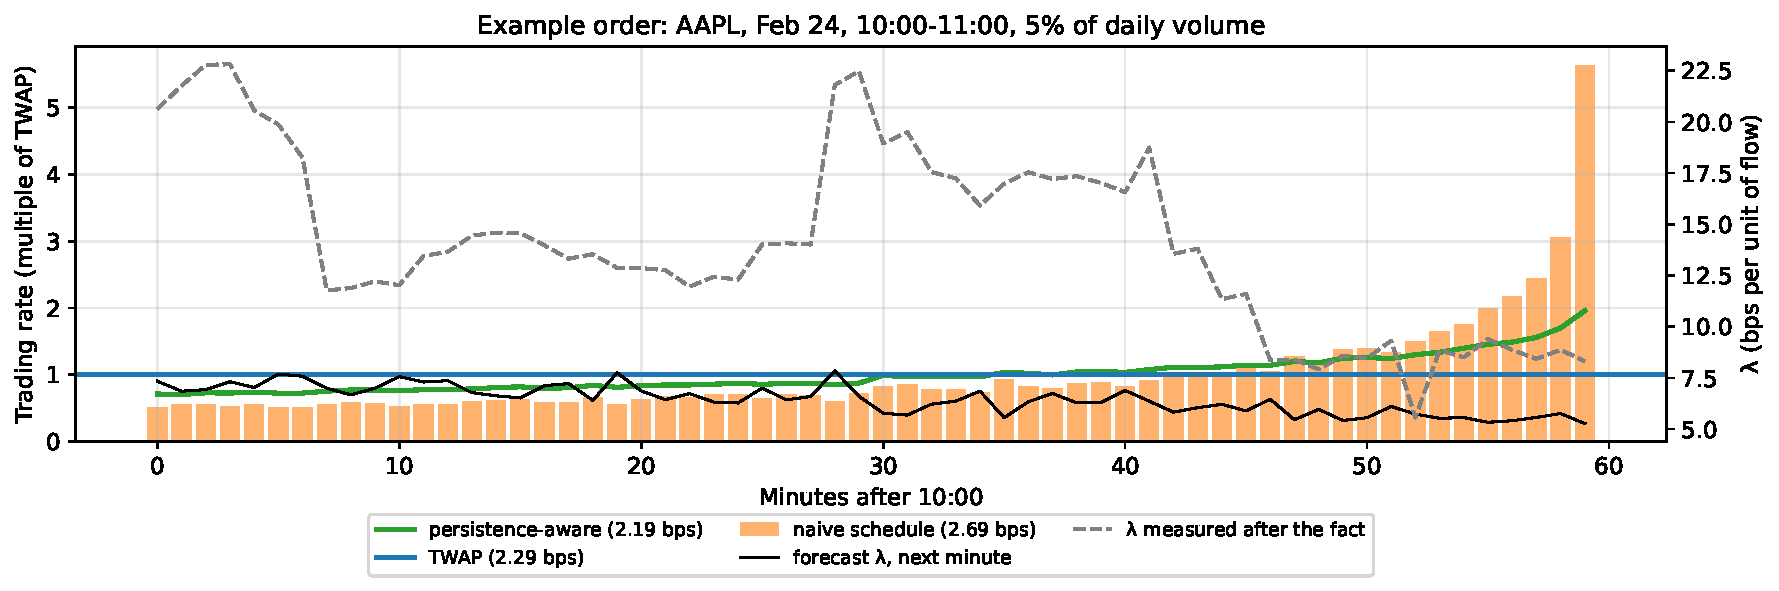
\includegraphics[width=0.92\textwidth]{../figures/fig4_example.pdf}
\caption{One order (AAPL, February 24, 10:00--11:00). The naive schedule sees high impact now, waits for it to fall, then buys at five times the TWAP rate in the last minutes; the persistence-aware schedule stays close to TWAP.}\label{fig:example}
\end{figure}

\begin{table}[h]
\centering\small
\caption{Execution results, test days, orders of 5\% of daily volume over one hour. Left: average cost of each schedule (bps). Right: accuracy of pre-trade cost estimates (bps); the last column is the change in mean squared error against the stock's usual cost ($t$-statistic, clustered by date).}\label{tab:exec}
\setlength{\tabcolsep}{4pt}
\begin{tabular}{lccc@{\hskip 14pt}lcccc}
\toprule
\multicolumn{4}{l}{\textit{When to trade}} & \multicolumn{5}{l}{\textit{How much the order will cost}} \\
Schedule & Calm & Sell-off & vs.\ TWAP & Estimate & RMSE & Bias & Corr. & vs.\ usual cost \\
\midrule
TWAP & 1.14 & 1.50 & -- & Single constant & 1.09 & 0.26 & -- & $+0.39$ (5.9) \\
Time-of-day pattern & 1.15 & 1.50 & +0.5\% & Stock's usual cost & 0.89 & 0.26 & 0.62 & -- \\
Naive, regression & 1.26 & 2.43 & +42.8\% & Time-of-day pattern & 1.09 & 0.26 & 0.01 & $+0.40$ (5.7) \\
Naive, boosting & 1.26 & 3.11 & +71.1\% & Usual cost $\times$ regression & \textbf{0.80} & 0.05 & \textbf{0.66} & $\mathbf{-0.15}$ ($-2.7$) \\
Persistence-aware, regression & 1.17 & 1.55 & +3.1\% & Usual cost $\times$ boosting & 0.83 & 0.01 & 0.62 & $-0.09$ ($-1.7$) \\
Persistence-aware, boosting & 1.15 & 1.52 & +1.2\% & & & & & \\
\bottomrule
\end{tabular}
\end{table}

\begin{figure}[h]
\centering
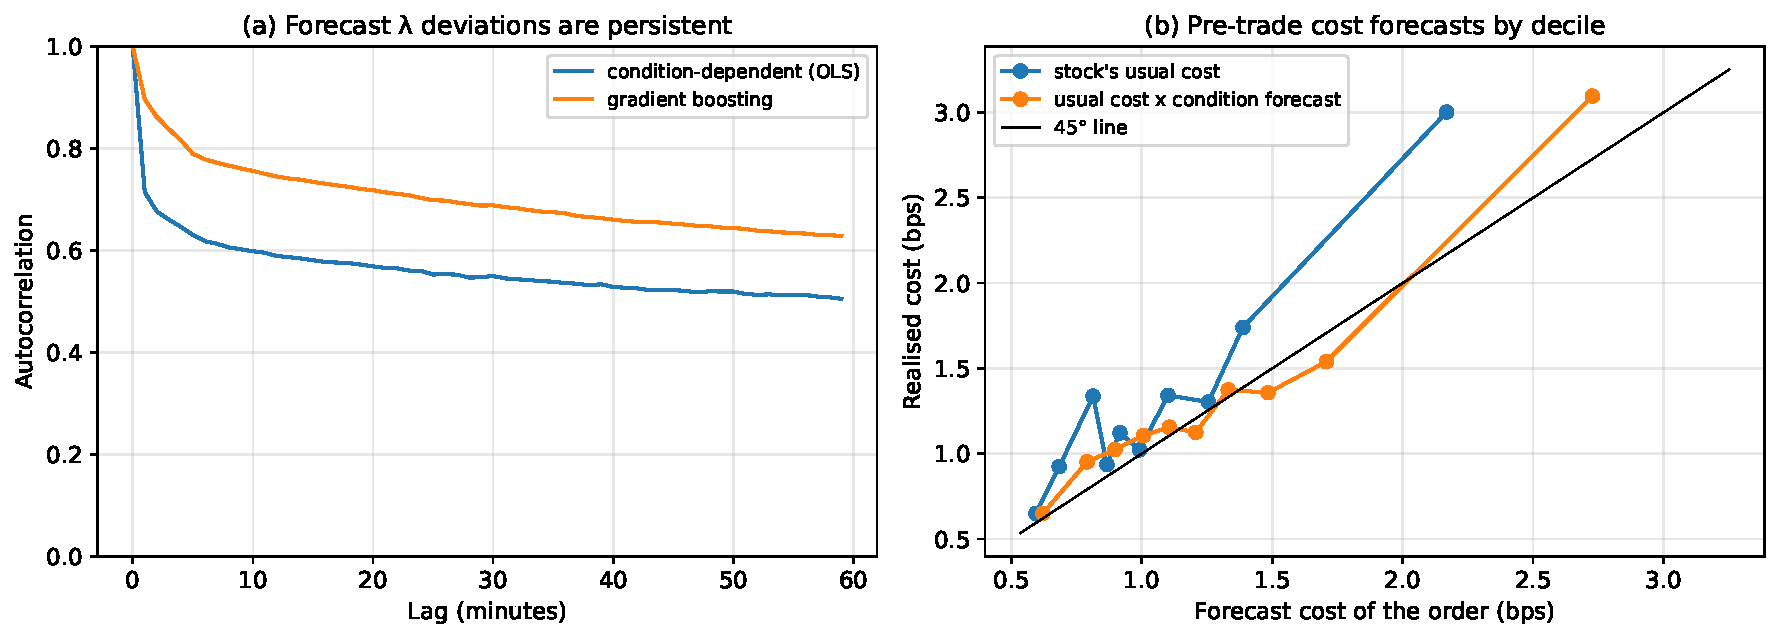
\includegraphics[width=0.92\textwidth]{../figures/fig5_value.pdf}
\caption{What the forecast is worth. (a) Deviations of the forecast from normal persist for over an hour, so the forecast says little about which minute is cheaper. (b) Realised against estimated order cost by decile: the stock's usual cost misses the most expensive orders, and the condition-based estimate tracks them.}\label{fig:worth}
\end{figure}

\textit{A note on market impact.} Our cost model treats one-minute impact as temporary. If it were permanent, the same order would cost about 81 bps, which is implausible for 5\% of daily volume; most of the one-minute move must therefore reverse. Our own orders would also widen spreads and shift order-flow imbalance, changing the very conditions we forecast from, a feedback that historical data cannot show.

\section{Conclusion}
\begin{itemize}
\item \textbf{What moves impact:} only unexpected flow; impact is highest at the open; wide spreads raise it and deep books lower it, as classic theory predicts.
\item \textbf{Forecasting:} conditions observed a minute earlier improve out-of-sample forecasts of impact. Most of what a machine-learning model adds is that impact grows more slowly than order size, which one regression term captures.
\item \textbf{Value to a trader:} high impact persists, so the forecast does not help to time trades within an hour; it does help to estimate an order's cost, which drives order sizing and participation limits.
\item \textbf{Limitations:} 19 days of data ending in a regime change; best quotes only (no view of the order book behind them); some trades misclassified by the Lee--Ready rule; simulated rather than actual execution.
\item \textbf{Extensions:} a risk-averse schedule (Almgren and Chriss, 2000), where the level of $\lambda$ changes how fast to trade; full order-book data to measure how quickly liquidity refills; and common factors in $\lambda$ across stocks (Hasbrouck and Seppi, 2001).
\end{itemize}

\section*{References}
\footnotesize
\setlength{\parskip}{1pt}
Admati, A. and Pfleiderer, P. (1988). A theory of intraday patterns: volume and price variability. \emph{Review of Financial Studies} 1(1), 3--40.\\
Almgren, R. and Chriss, N. (2000). Optimal execution of portfolio transactions. \emph{Journal of Risk} 3(2), 5--39.\\
Cont, R., Kukanov, A. and Stoikov, S. (2014). The price impact of order book events. \emph{Journal of Financial Econometrics} 12(1), 47--88.\\
Diebold, F. and Mariano, R. (1995). Comparing predictive accuracy. \emph{Journal of Business \& Economic Statistics} 13(3), 253--263.\\
Glosten, L. and Milgrom, P. (1985). Bid, ask and transaction prices in a specialist market with heterogeneously informed traders. \emph{Journal of Financial Economics} 14(1), 71--100.\\
Hasbrouck, J. (1991). Measuring the information content of stock trades. \emph{Journal of Finance} 46(1), 179--207.\\
Hasbrouck, J. and Seppi, D. (2001). Common factors in prices, order flows, and liquidity. \emph{Journal of Financial Economics} 59(3), 383--411.\\
Ke, G. et al. (2017). LightGBM: a highly efficient gradient boosting decision tree. \emph{Advances in Neural Information Processing Systems} 30.\\
Kwan, A., Philip, R. and Shkilko, A. (2021). The conduits of price discovery: a machine learning approach. Working paper, SSRN 3710491.\\
Kyle, A. S. (1985). Continuous auctions and insider trading. \emph{Econometrica} 53(6), 1315--1335.\\
Lee, C. and Ready, M. (1991). Inferring trade direction from intraday data. \emph{Journal of Finance} 46(2), 733--746.\\
Lundberg, S. and Lee, S.-I. (2017). A unified approach to interpreting model predictions. \emph{Advances in Neural Information Processing Systems} 30.\\
T\'oth, B. et al. (2011). Anomalous price impact and the critical nature of liquidity in financial markets. \emph{Physical Review X} 1, 021006.
\end{document}
